\chapter{Introduction}
\label{chap:intro}

\begin{figure}
\caption{The Internet's four-layer stack model}
\label{f:stack}
\begin{centering}
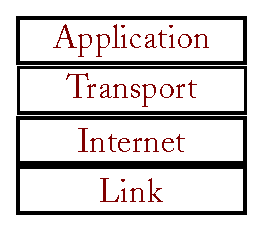
\includegraphics{layers.pdf}

\end{centering}
\end{figure}

\begin{figure}
\caption{As the Internet has evolved, researchers have created at
  least 40 mechanisms to govern resource allocation on the
  network---both entirely distributed schemes (``end-to-end'') and
  ones that include code running ``in-net.''}
\label{f:march}

\vspace{\baselineskip}

\begin{centering}
\noindent 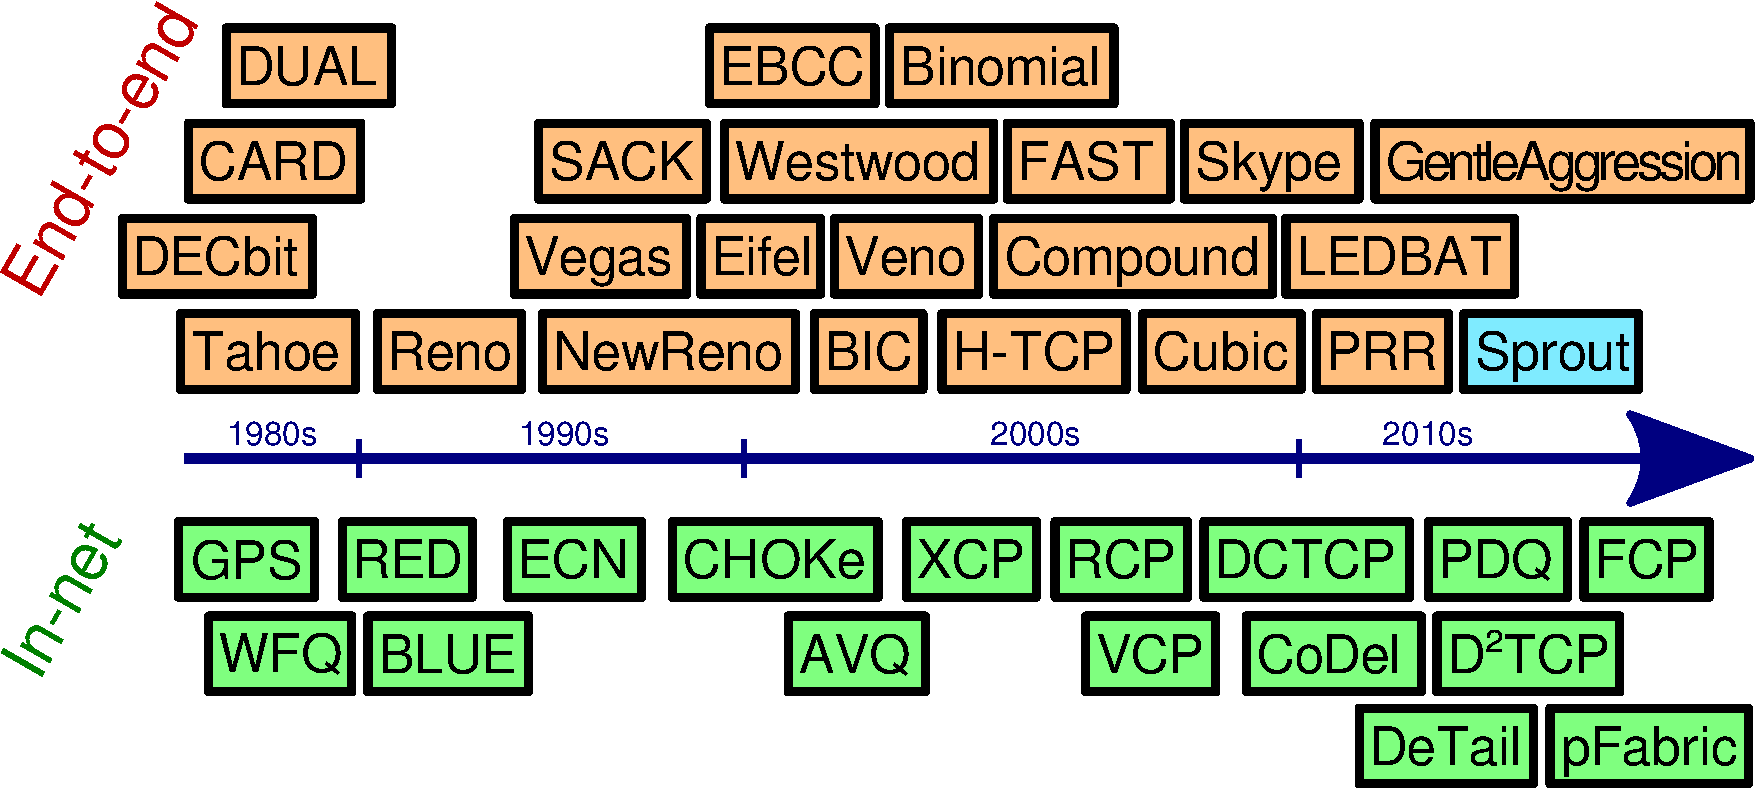
\includegraphics[width=\textwidth]{march2-all.pdf}

\end{centering}
\end{figure}

Over the last 25 years, the Internet has transformed from an academic
networking experiment into a global utility with billions of
users. With this rise, every layer of the Internet
``stack'' has seen dramatic change.

At the \textbf{link} layer, technologies that did not exist 25 years
ago now dominate---including wireless local-area networks (Wi-Fi),
cellular networks, datacenter interconnects, and transoceanic links
with high delay.

One layer up, at the \textbf{Internet} layer, mobility is now
ubiquitous. User devices regularly change their interface IP addresses
as they roam from network to network.

At the top layer of the Internet stack---the \textbf{application}
layer---none of the dominant applications of today existed 25 years
ago, including the World Wide Web and its short flows,
progressive-download video applications (e.g., YouTube and Netflix),
and real-time streaming video (e.g., Skype and Facetime).

The whole Internet has had to grapple with this continuous
evolution. How should the protocols of the \textbf{transport} layer,
sitting in the middle of the stack between the application and the
Internet, adapt to evolving application demands above them and
evolving networks below?

One legitimate answer is that these transport-layer protocols won't be
asked to adapt at all. If the network or applications evolve, our
current protocols will either be acceptable or not when run on the new
network or in service of the new application. If a protocol works
adequately, all is well. If not, we can simply stop using the protocol
and design a fresh one that matches the new circumstances.

This approach may sound wasteful, but it describes the extraordinarily
successful path taken over the last 25 years. Looking at just one
function of the transport layer---congestion control, the job of
dividing up the network's resources among contending
users---researchers have accommodated new applications and network
behaviors by devoting considerable effort to develop newer and newer
mechanisms, at least 40 in total so far (Figure \ref{f:march}).

Despite its demonstrable success, this approach can have downsides. In
defining transport-layer protocols by their \emph{mechanisms}---by the
actual behavior of endpoints or gateways that execute the
protocol---we leave implicit the assumptions that the mechanism makes
about the behavior of other layers and the policy that the mechanism
is built to pursue.

For contemporary mechanisms (e.g., TCP Cubic, the current default in
Linux), it's difficult to state the assumptions that the transport
makes about lower layers and to predict when those assumptions would
no longer hold. This presents a challenge for link-layer designers who
wish to design a new networking technology. Because of Cubic's
popularity, it can be a \emph{de facto} requirement that Cubic perform
well over any new network. In effect, this means that the designer of
the new link layer must try to satisfy Cubic's implicit assumptions in
order to achieve adequate performance.

This has led to the ``bufferbloat''\cite{bufferbloat} problem, which
comes from a link layer's attempt to hide losses from the transport,
on the grounds that the transport will assume that losses are a signal
to slow down. It has also led to a lack of parallelism in Internet
routing---flows only take one path, even if speedups might be
available by splitting flows across multiple routes---on the grounds
that the transport protocol probably assumes that out-of-order packets
are a pathology.

On the flip side, it is nontrivial to adjust the assumptions made by
the transport layer. There's no clear way to tweak the assumptions and
then retrace the same design process that was followed by a protocol's
designers, in order to explore the mechanism they would have produced
given a different starting point.

\section{The benefits of showing our work as designers}

This thesis proposes essentially that approach to protocol design. The
transport layer should adapt to whatever the layers below may do, and
whatever the application above it wants done. Protocol designers
should specify the \emph{policy}---namely, what assumptions they want
to make about the network and what kind of performance the application
is interested in---and let computers worry about translating that into
the mechanism of congestion control.

By ``showing our work'' in this way, clearly enough for a computer to
recreate the same design, altering the assumptions is a matter of
changing the inputs to a computer program. This makes it easier for
adjacent layers to evolve. My colleagues and I have also found that
this approach can yield better performance than conventional,
human-designed protocols.

Over the last three years, my colleagues and I have built a series of
systems to explore this approach:

\textbf{Mosh} (mobile shell)~\cite{mosh} is a replacement for SSH
(secure shell) in which the client and server each explicitly model
the dynamic contents of the text terminal. Unlike SSH, which transmits all
output from an application through a reliable TCP connection and
doesn't attempt to interpret the stream, Mosh's modeling allows it
to choose which data to send to the client when, in order to most
efficiently satisfy an explicit objective: update the client screen to
the current contents of the text terminal as efficiently as possible,
even across intermittent, roaming connectivity.

Mosh is primarily a remote terminal application and is not further
discussed in this dissertation, but its design ideas---maintain an
explicit model at runtime, and pursue a stated objective on behalf
of the user---formed the basis of our subsequent work on transport
protocol design.

\textbf{Sprout} (Chapter~\ref{chap:sprout}) is a transport protocol
designed to carry high-throughput interactive traffic, such as a
videoconference, over a cellular network. Sprout includes an explicit
model of the dynamics of cellular networks and makes predictions about
future network performance by inferring, with uncertainty, the current
state of the network and evolving the model forward. Its control
strategy---how much data to send at a given moment---is a function of
those predictions and of an explicit objective: maximize throughput,
but bound in-network delays to be at most 100~ms with high
probability. On commercial cellular networks, Sprout gives 2-to-4
times the throughput and 7-to-9 times less delay than Skype, Apple
Facetime, and Google Hangouts.

\textbf{Remy} (Chapter~\ref{chap:remy}) expands Sprout to the
classical problem of \emph{multi-agent} congestion control, where many
applications may contend for the same limited network resource. Remy
is a protocol-design tool that takes, as input, a set of assumptions
about the uncertain network and workload, and an objective to pursue
on behalf of the application. Remy's computer-generated algorithms can
achieve higher performance and greater fairness than some
sophisticated human-designed schemes, including ones that put
intelligence inside the network.

Once we had a computerized protocol designer, we explored using it as
a tool to gain understanding about the problem of congestion control.
How easy is it to ``learn'' a network protocol to achieve desired
goals, given a necessarily imperfect model of the networks where it
ultimately will be deployed? Is there a tradeoff between the
performance of an algorithm now---if optimized for a very specific
network---versus the protocol's ability to perform adequately as the
network evolves? What is the cost of compatibility with existing TCP
congestion-control mechanisms? Our experimentation into these
questions of ``learnability'' is reported in
Chapter~\ref{chap:learnability}.
